\section{Discriminant Variables}\label{sec-vh-disc}
The analysis leverages a varied set of reconstructed physical variables in the fit to constrain the different processes and control mis-modelling effects. Figure \ref{fig:variablesControlReg} displays the variables used for each control region in the fit in the resolved regime. The reconstructed Higgs mass directly offer some separation power of the signals from their major backgrounds, hence some control regions such as the Top $BT$ \gls{cr} and CRHigh are modelled with these relevant variables: $m_{bb}$, $m_{cc}$, and $m_J$, depending on the targeted decay and the regime. Some \gls{cr}s passed to the fit are modelled with the $p_T^V$ distribution, such as the CRHigh in the 2L-channel $NT$ and $BB$ tagged-regions and the $V+l$ \gls{cr} ($LN$-tag). Directly fitting this distribution helps constrain a Monte-Carlo mis-modelling in the \ptv\ distributions of the \textsc{Sherpa} 2.2.11 $V+$jets samples, as detailed in Section \ref{sec-mod}. To optimise signal and background seperation in the statistical analysis, dedicated \gls{bdt}, also called \gls{mva}, are trained with the \textsc{TMVA} Root framework \cite{Therhaag:2011jh} in the signal regions of the combined analysis. Simple one-dimensional discriminants are built from the outputs of fine-tuned \gls{bdt}s trained on specific sets of event-level input variables, as described in greated details in this section. \\

\subsection{Multivariate Analysis}
Three sets of discriminants are trained for the analysis: one set of called \textit{\gls{mva}} discrimants for the signal region modelling, and a specific set called \textit{mvaCRLow} for the CRLow distribution in the resolved \vhb. An additional set of \gls{bdt}s is trained for the cross-check analysis targetting the diboson process as signal, where one of the bosons is a $Z$ ($WZ$ or $ZZ$n summarised as $VZ$) with a $b\bar{b}$ or $c\bar{c}$ pair in the final state. For this purpose, the signal is set to the diboson process decayig into the expected pair of jets $VZ(\rightarrow b\bar{b})$ or $VZ(\rightarrow c\bar{c})$, and the non diboson processes as well as the $VH$ processes are set as backgrounds. All multivariate discriminants predict a continous score in the range $[-1, 1]$, with higher values indicating a signal-like component and lower values background-like.

\begin{figure}[h!]
  %\hspace{-2.0cm}
  \center
  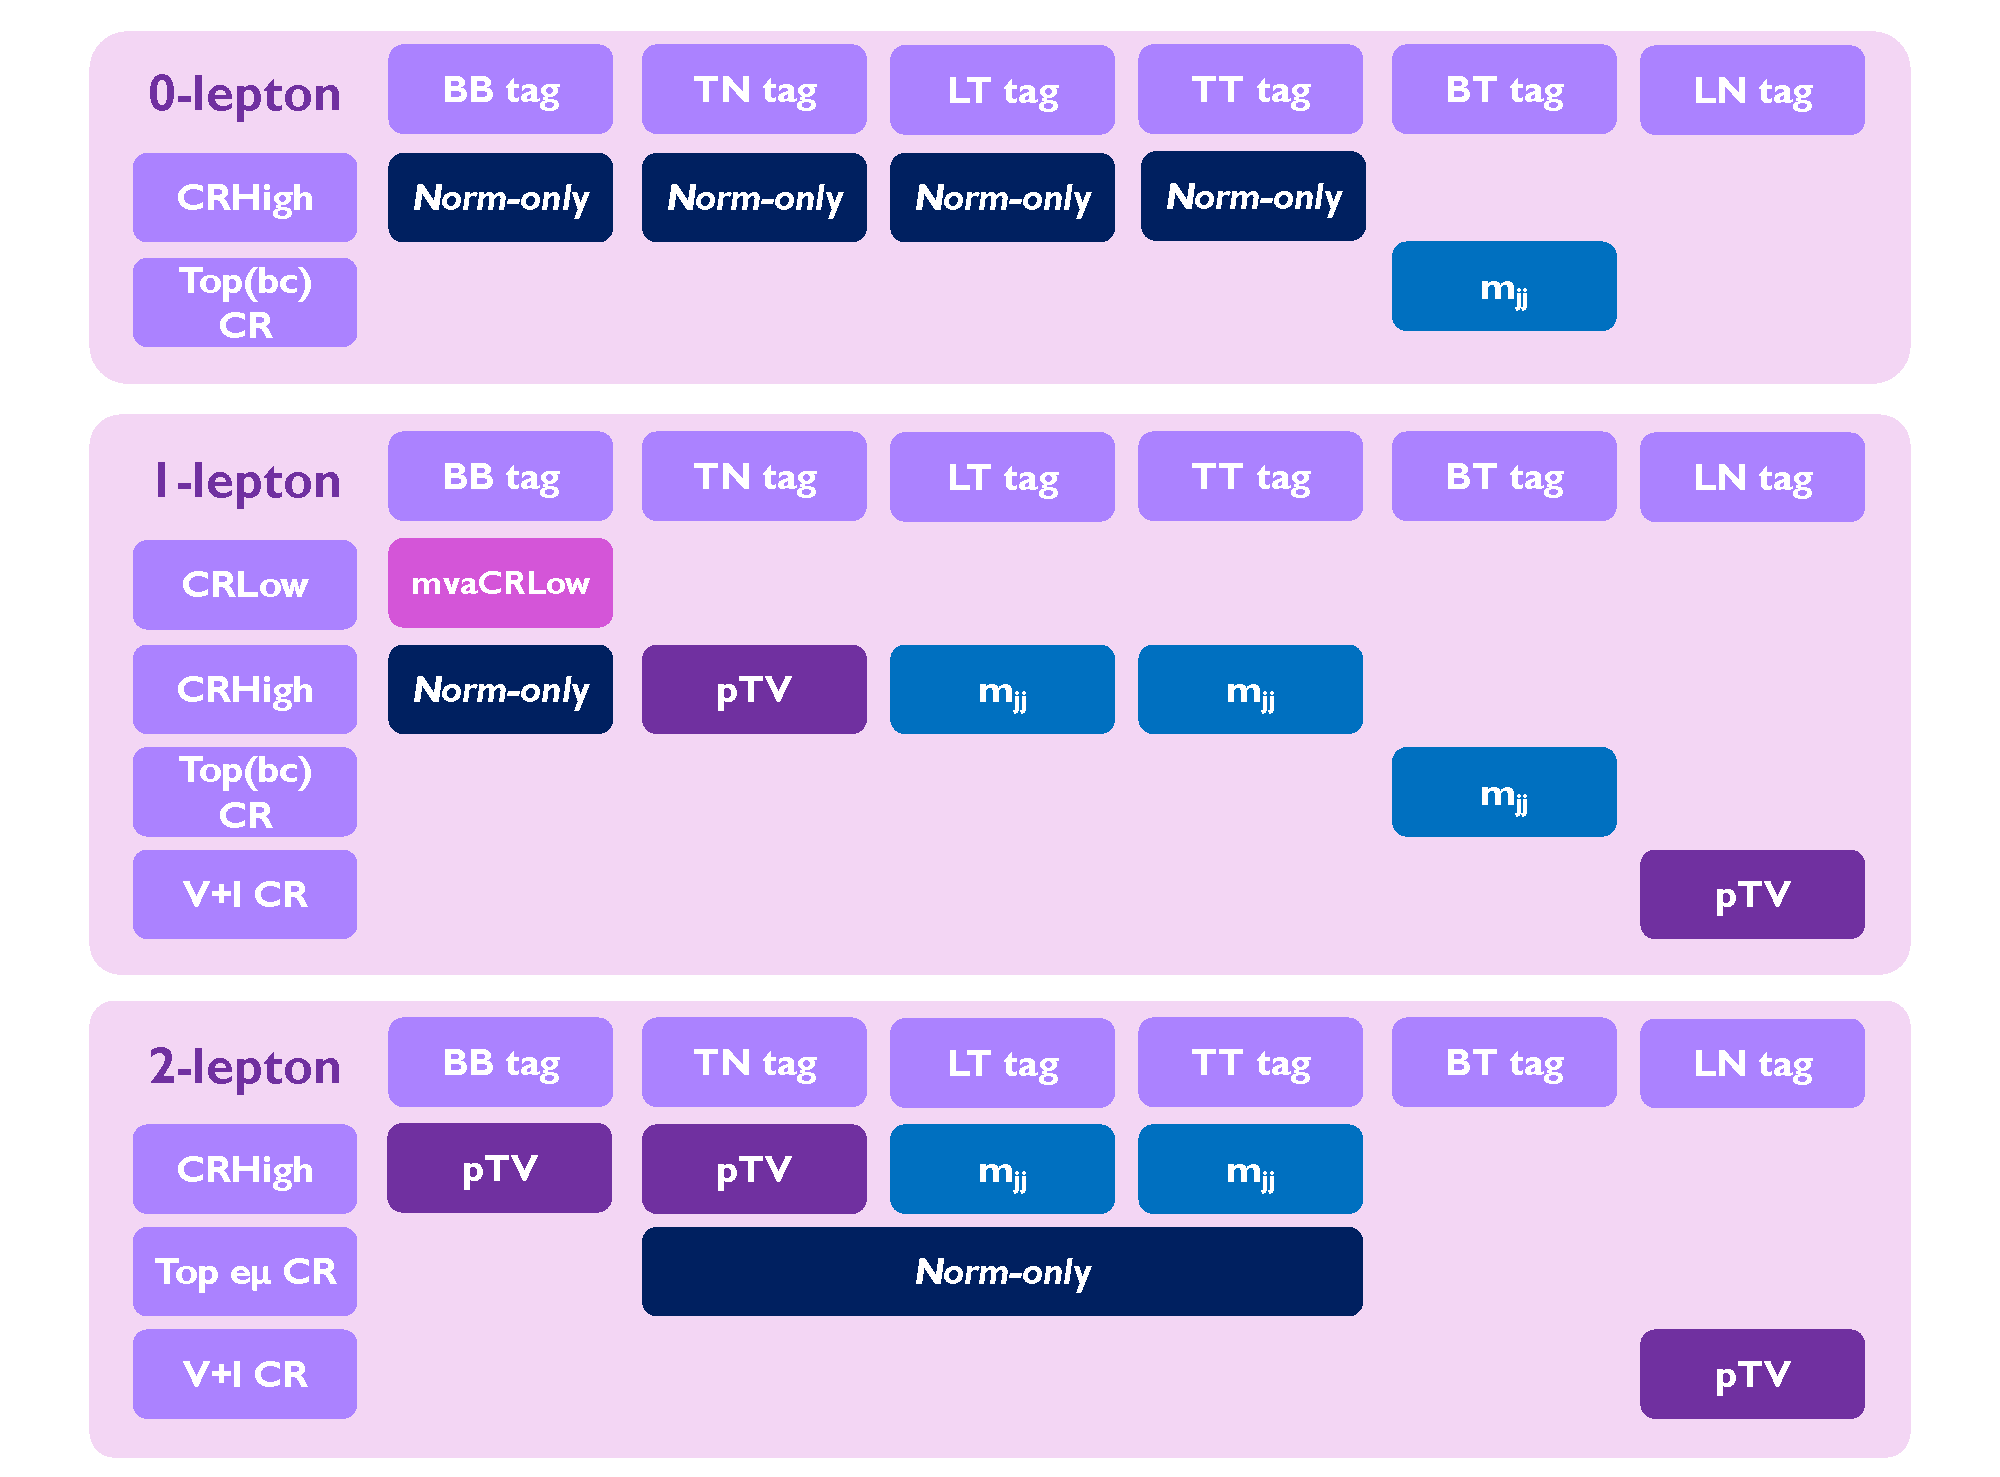
\includegraphics[width=0.98\textwidth]{Images/VH/Discriminants/Variables.pdf}
  \caption{Illustration of the discriminant variables used per control regions of the resolved regime in the fit. Norm-only indicates a region to extract a global normalisation and not binned by a variable.} % Maybe re-do it yourself ...
  \label{fig:variablesControlReg}
\end{figure}

The wide-adoption of \gls{bdt}-discriminants in all regime of the analysis marks a significant improvement over the standalone \vhc\ and boosted \vhb\ analyses, generalising the successful approach first introduced in the resolved \vhb\ \cite{ATLAS:2020fcp}. Prior to training, the object and event selections of Section \ref{sec-selectionandcat} and the jet energy corrections of Section \ref{sec-vh-jetcor} are applied. To limit the number of training runs and the risk of overtraining from the low statistics of some kinematic regions, the \gls{bdt}s are trained on inclusive regions combining the \gls{sr}s and the $\Delta R$-based \gls{cr}s (CRHigh and CRLow). The \gls{bdt}s are trained to discriminate the respective signal of the different targeted decays \footnote{The \vhb\ samples for the $BB$-tagged events and \vhc\ samples for the 1 and 2 $c$-tagged events.} from background samples, including $V+$jets, \ttb, single-top, and diboson. \gls{bdt}s were specifically trained in the following specific categories, covering the fine analysis categorisation with different categories limits to guarantee sufficient statistics and avoid overtraining:
\begin{itemize}[leftmargin=*]
  \item \textbf{Resolved \boldvhbc:} \gls{bdt}s are trained separately for the $BB$-, 2 $c$- ($TT+TL$ abbreviated $XT$), and 1 $c$-tags ($NT$). Seperate trainings are run for each lepton channel and for the following jet multiplicities\footnote{The jet multiplicity only accounts for jets with $p_T > 30$ GeV.} and \ptv\ bins:
  \begin{itemize}
      \item \textbf{0L}: separate \gls{bdt}s are trained for the 2-, 3-, and 4-jet categories, each in one inclusive \ptv\ $\geq 150$ GeV region.
      \item \textbf{1L}: separate \gls{bdt}s are trained for the 2- and 3-jet categories, each in two \ptv\ bins: \ptv\ $\in [75, 150]$ GeV and \ptv\ $\geq 150$ GeV.
      \item \textbf{2L}: separate \gls{bdt}s are trained for the 2- and $\geq$3-jet categories in two \ptv\ bins: \ptv\ $\in [75, 150]$ GeV and \ptv\ $\geq 150$ GeV.
  \end{itemize}
  The low \ptv\ bin is separated from the higher \ptv\ $>$ 150 GeV due to its large statistics and different background compositions.
  \item \textbf{Boosted \vhb:} one \gls{bdt} is trained per lepton channel in an inclusive bin of \ptv\ $\geq$ 400 GeV.
\end{itemize}

For training, the full \gls{mc} samples statistics in all analysis regimes are used thanks to the so-called \textit{GNN truth tagging}. Instead of filtering down the simulated samples by cutting away events failing to pass the flavour tagging requirements - the standard application of the selection called \textit{direct tagging} -, this technique applies a weight to each event to represent its probability of passing the tagging selection. The result is a weighted distribution possessing the statistical precision of the full \gls{mc}-samples but shaped as the directly tagged distributions. The weights in this truth tagging procedure are predicted by a \gls{gnn}-based neural network passed event-level information, with more details given in Appendix \ref{app-truth-tagging}. The truth tagging procedure is applied to $BB$ for \vhb, and to $TT$, $TL$, and $NT$ for \vhc. The variables used for each lepton channel in both regimes are listed in Table \ref{tbl:MVAVars}, with more precise definitions of each variable given in Appendix \ref{ap-MVA}. Features with long tails are clipped to contain 99\% of the centred distributions, and given a specifically chosen default value when they are not defined for an event. The sets of features used are the result of hyperparameter optimisation campaigns, with many other variables tested but eventually not included due to their negligible impact on the performance. 

\begin{table}[!htbp]
    \hspace{-1cm}
    %\renewcommand*{\arraystretch}{1.3}
    \newcommand\textunderset[2]{\ensuremath{\underset{\textrm{#1}}{\textrm{#2}}}}
      %\setlength\aboverulesep{0pt}
      %\setlength\belowrulesep{0pt}
      % resize a bit the table 
      %\resizebox{1\textwidth}{!}{ %
      \begin{tabular}{c|ccc|ccc|M{6cm}}
        %\multicolumn{1}{c}{} & \multicolumn{3}{c}{\textunderset{Resolved}{\vhbc}} & \multicolumn{3}{c}{\textunderset{Boosted}{\vhb}} & \multicolumn{1}{c}{}
        \multicolumn{1}{c}{} & \multicolumn{3}{c|}{\vhbc} & \multicolumn{3}{c}{\vhb} & \multicolumn{1}{c}{}\\
        \multicolumn{1}{c}{} & \multicolumn{3}{c|}{Resolved} & \multicolumn{3}{c}{Boosted} & \multicolumn{1}{c}{}
        \\ \hline \hline
        Variable & 0L & 1L & 2L & 0L & 1L & 2L 
        \\ \hline
        $m_{j_1j_2}$ or $m_J$
            & \checkmark & \checkmark & \checkmark 
            & \checkmark & \checkmark  & \checkmark 
            & Mass of Higgs candidate
        \\ \hline
        $m_{{j_1 j_2 j_3}}$ 
            & \checkmark & \checkmark & \checkmark 
            & & &
            & Mass of Higgs candidates and leading additional jets
        \\ \hline
        $p_T^{j_1}$
            & \checkmark & \checkmark & \checkmark 
            & \checkmark & \checkmark & \checkmark 
            & Leading Higgs candidate $p_T$
        \\ \hline
        $p_T^{j_2}$
            & \checkmark & \checkmark & \checkmark 
            & \checkmark & \checkmark & \checkmark 
            & Subleading Higgs candidate $p_T$
        \\ \hline
        $p_T^{j_3}$ 
            & & & 
            & \checkmark & \checkmark & \checkmark 
            & Leading non-Higgs candidate $p_T$
        \\ \hline
        $\sum\limits_{i\neq 1, 2}p_T^{j_i}$ 
            & \checkmark & \checkmark & \checkmark 
            & & & 
            & Sum of non-Higgs jet $p_T$
        \\ \hline
        $\Delta R(\boldsymbol{j_1}, \boldsymbol{j_2})$
            & \checkmark & \checkmark & \checkmark 
            & \checkmark & \checkmark & \checkmark 
            & Angular separation of Higgs candidates
        \\ \hline
        $\mathrm{bin}_{\mathrm{DL1r}}(j_1)$ 
            & \checkmark & \checkmark & \checkmark
            & \checkmark & \checkmark & \checkmark 
            & Tag bin of $j_1$
        \\ \hline
        $\mathrm{bin}_{\mathrm{DL1r}}(j_2)$ 
            & \checkmark & \checkmark & \checkmark
            & \checkmark & \checkmark & \checkmark 
            & Tag bin of $j_2$
        \\ \hline
        \ptv 
            & $\equiv E_T^{\textrm{miss}}$ & \checkmark  & \checkmark
            & $\equiv E_T^{\textrm{miss}}$ & \checkmark  & \checkmark
            & Vector boson $p_T$
        \\ \hline
        $E_T^{\textrm{miss}}$
            & \checkmark & \checkmark & 
            & \checkmark & \checkmark & 
            & Missing transverse energy
        \\ \hline
        $E_T^{\textrm{miss}}/\sqrt{S_T}$
            & & & \checkmark 
            & & & 
            & Ratio of \etm\ to sum of jets $p_T$
        \\ \hline
        $|\Delta y(\boldsymbol{V},\boldsymbol{H})|$
            & & \checkmark & \checkmark
            & & \checkmark & \checkmark
            & Rapidity between $V$ and $H$
        \\ \hline
        $|\Delta \phi(\boldsymbol{V},\boldsymbol{H})|$
            & \checkmark & \checkmark & \checkmark
            & \checkmark & \checkmark & \checkmark
            & Azimuthal angle between $V$ and $H$
        \\ \hline
        $|\Delta \eta(\boldsymbol{j_1},\boldsymbol{j_2})|$
            & \checkmark & & 
            & & & 
            & Pseudorapidity distance between Higgs candidates
        \\ \hline
        $\min\Delta R(j_i, j)_{i=1,2}$
            & \checkmark & \checkmark & 
            & & & 
            & Smallest angular distance between a Higgs and non-Higgs candidates
        \\ \hline
        $\mathrm{min}[\Delta\phi(\boldsymbol{\ell},\boldsymbol{j_1} \textrm{~or~} \boldsymbol{j_2})]$
            & & \checkmark  &
            & & & 
            & Smallest $\phi$ between the lepton and a Higgs candidate
        \\ \hline
        $m_{\textrm{eff}}$
            & \checkmark & & 
            & & &
            & Scalar sum of $p_T$ of all small-$R$ jet and \etm
        \\ \hline
        $m_T^W$
            & & \checkmark &
            & & &
            & Transverse mass of the $W$
        \\ \hline
        $m_{\textrm{top}}$
            & & \checkmark &
            & & &
            & Mass of reconstructed top-quark decaying semi-leptonically
        \\ \hline
        $m_{\ell\ell}$
            & & & \checkmark 
            & & & 
            & Mass of di-lepton system
        \\ \hline
        $\cos{\theta(\boldsymbol{\ell^-},\boldsymbol{Z})}$
            & & & \checkmark 
            & & & \checkmark 
            & $Z$ boson polarisation sensitive angle
        \\ \hline
        $(p_T^{\ell_1} - E_T^{\textrm{miss}})/p_T^W$
            & & &
            & & \checkmark & 
        \\ \hline
        $p_T^{\ell}$
            & & &
            & & \checkmark & 
            & \pt\ imbalance of the lepton and neutrino from $W$ 
        \\ \hline
        $N(\textrm{track-jets in }J)$
            & & & 
            & \checkmark & \checkmark & \checkmark
            & Number of track-jets associated to leading-$R$ jet
        \\ \hline
        $N(\textrm{add. small R-jets})$
            & & & 
            & \checkmark & \checkmark & \checkmark
            & Number of additional small-$R$ jets not matched
        \\ \hline
        Colour
            & & & 
            & \checkmark & \checkmark & \checkmark
            & Variable modelling colour-flow from \gls{qcd}
        \\ \hline \hline
      \end{tabular}
      %}
      \caption{%
        The variables used for the 0L, 1L, and 2L channels MVA's in the resolved and boosted regimes for the \vhbc\ combined analysis. The variables are further described in Appendix \ref{ap-MVA}.}%
      \label{tbl:MVAVars}
    \end{table}
  

The architectures of the different \gls{bdt}s are optimised, with the gradient boosting technique of Section \ref{sec-gradient-boost} deployed in the resolved regime to improve performance and to capture effects outside the bulk of the distributions. In the boosted regime, due to the lower statistics available and large tails in the distributions, the AdaBoost method - introduced in Section \ref{sub-adaboosted} - is adopted to help stabilise the trainings \cite{Adaboost}. Tables \ref{tbl:MVAHyperparams} and \ref{tbl:MVAHyperparams-VHcc} list the architectures used for the \vhb\ and \vhc\ \gls{bdt}s respectively, with the main and diboson \gls{bdt}s sharing the same hyperparameters. For \vhc, the hyperparameters are further tuned to avoid overtraining from the smaller available statistics in the 2L channel and the diboson cross-check.

\begin{table}[!htbp]
  \renewcommand*{\arraystretch}{1.3}
  \newcommand\textunderset[2]{\ensuremath{\underset{\text{#1}}{\text{#2}}}}
  \centering
    % resize a bit the table 
    \resizebox{1\textwidth}{!}{%
    \begin{tabular}{c|ccc|ccc}
      \multicolumn{1}{c}{} & \multicolumn{3}{c|}{Resolved \vhb} &  \multicolumn{3}{c}{Boosted \vhb} 
      \\\hline \hline
      \textbf{Settings} & 0L & 1L & 2L & 0L & 1L & 2L
      \\\hline
      Boost type 
        & Gradient boost & Gradient boost & Gradient boost % VHbb Resolved 
        & Adaboost       & Adaboost       & Adaboost       % VHbb Boosted 
      \\\hline 
      Number of trees 
        & 200 & 600 & 200 % VHbb Resolved 
        & 800 & 800 & 400 % VHbb Boosted 
      \\\hline 
      Maximum depth
        & 3 & 4 & 4 % VHbb Resolved 
        & 3 & 3 & 3 % VHbb Boosted 
      \\\hline 
      Learning rate ($\beta$) 
        & 0.5 & 0.5 & 0.5% VHbb Resolved 
        & 0.5 & 0.35 & 0.3 % VHbb Boosted 
      \\\hline 
      Number of cuts
        & 100 & 100 & 100% VHbb Resolved 
        & 60  & 60  & 100 % VHbb Boosted 
      \\\hline 
      Minimum node size 
        & 5\% & 5\% & 5\% % VHbb Resolved 
        & 2\% & 2\% & 7\% % VHbb Boosted 
      \\ \hline \hline
    \end{tabular}}%
  \caption{%
    Hyperparameters of the BDTs in the 0L, 1L and 2L channels for the \vhb resolved and boosted. All models used the Gini index as separation method, without pruning.}%
  \label{tbl:MVAHyperparams}
\end{table}


% VHcc use different hyper parameters
\begin{table}[!htbp]
  \renewcommand*{\arraystretch}{1.3}
  \newcommand\textunderset[2]{\ensuremath{\underset{\text{#1}}{\text{#2}}}}
  \centering
    % resize a bit the table 
    %\resizebox{1\textwidth}{!}{%
    \begin{tabular}{c|cc|c}
      \multicolumn{1}{c}{} & \multicolumn{2}{c|}{\vhc} &  $VZ{\rightarrow c\bar{c}}$ signal
      \\\hline \hline
      \textbf{Settings} & 0L, 1L and most 2L regions & 2  3p-jet, low pTV & 0L, 1L and 2L
      \\\hline
      Boost type 
        & Gradient boost & Adaboost % VHcc
        & Adaboost                  % VZcc
      \\\hline 
      Number of trees 
        & 600 & 200 % VHcc
        & 200       % VZcc 
      \\\hline 
      Maximum depth
        & 4 & 4     % VHcc
        & 4         % VZcc
      \\\hline 
      Learning rate ($\beta$) 
        & 0.5 & 0.15 % VHcc
        & 0.15       % VZcc 
      \\\hline 
      Number of cuts
        & 100 & 100  % VHcc
        & 100        % VZcc
      \\\hline 
      Minimum node size 
        & 5\% & 5\%  % VHcc
        & 5\%        % VZcc
      \\ \hline \hline
    \end{tabular}
  %}
  \caption{%
    Hyperparameters of the BDTs in the 0L, 1L and 2L channels of \vhc. The 2L low pTV region mentioned is 75 GeV $<$ pTV $<$ 150 GeV. All models used the Gini index as separation method, without pruning.}%
  \label{tbl:MVAHyperparams-VHcc}
\end{table}


\begin{figure}[h!]
    \hspace{-0.3cm}
    \begin{subfigure}[b]{0.49\textwidth}
        \centering
      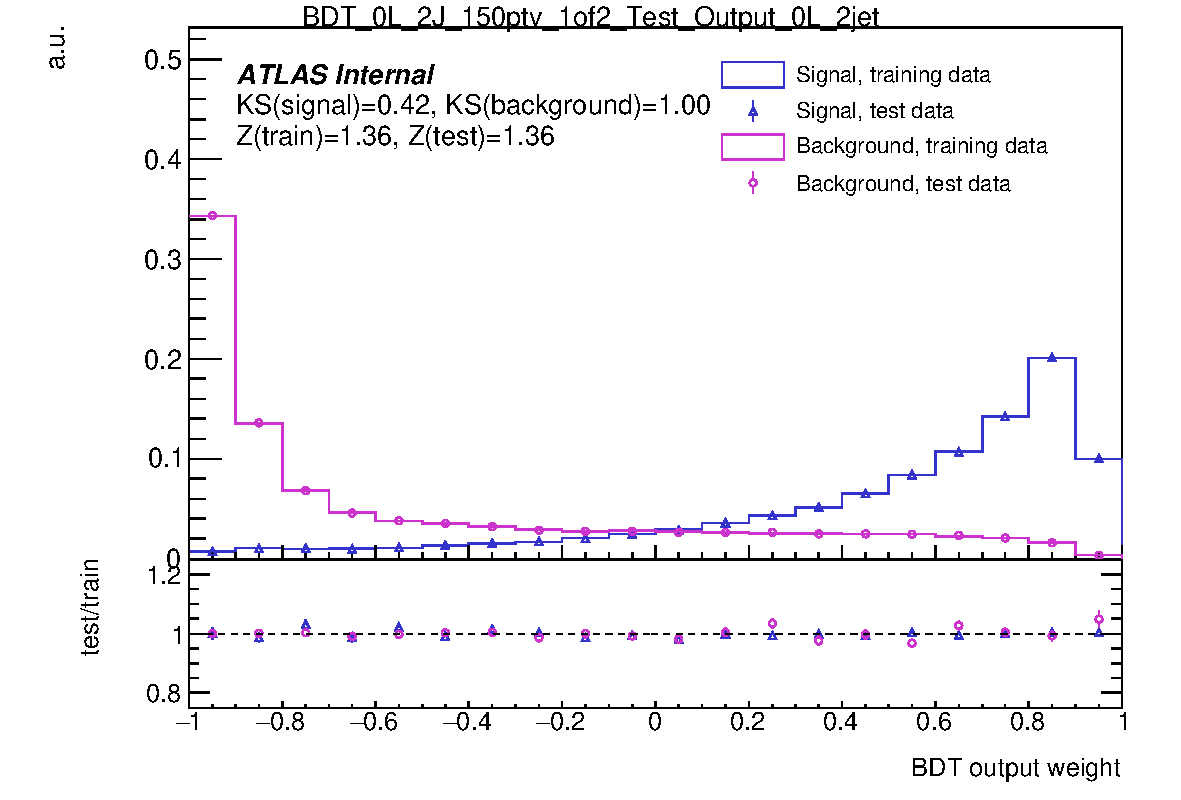
\includegraphics[width=\textwidth]{Images/VH/Discriminants/OvertrainCheck_BDT_0L_2J_150ptv_1of2_Test_Output_0L_2jet.pdf}
    \caption{$BB$-tagged model, test AUC = 0.9.} 
    \end{subfigure}
    \begin{subfigure}[b]{0.49\textwidth}
        \centering
      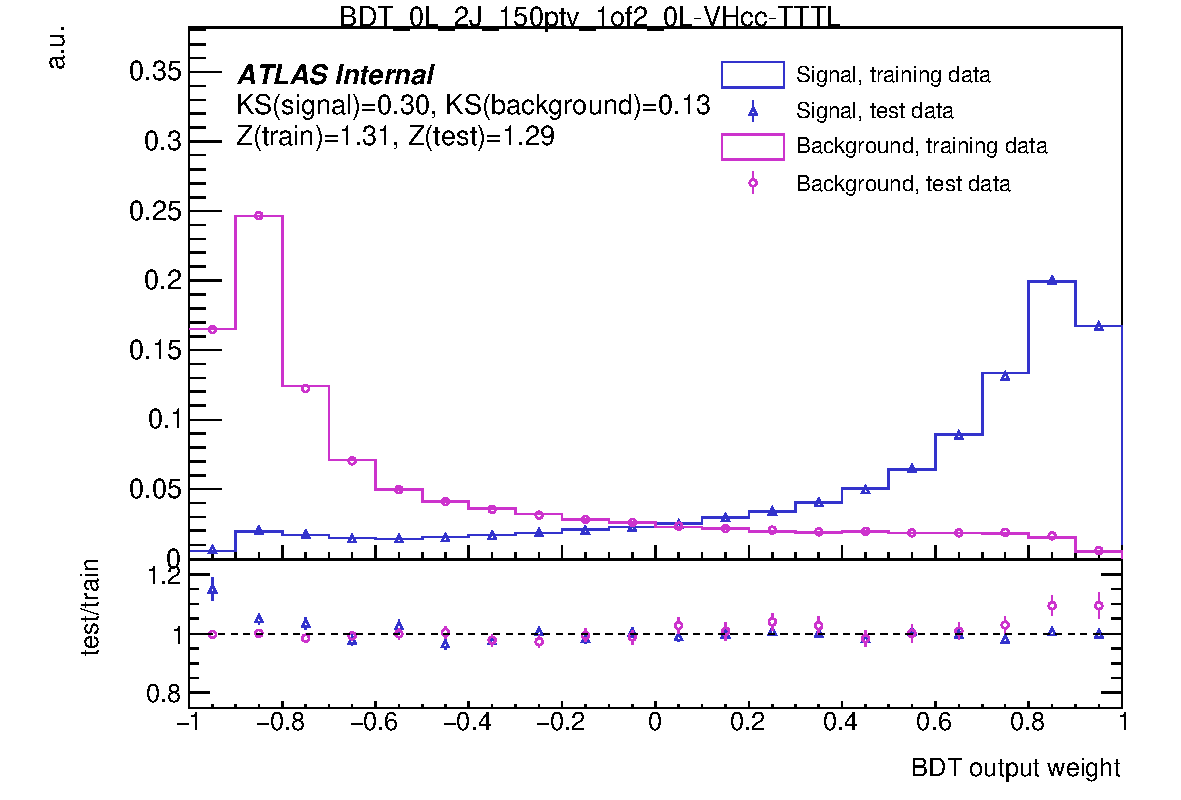
\includegraphics[width=\textwidth]{Images/VH/Discriminants/OvertrainCheck_BDT_0L_2J_150ptv_1of2_0L-VHcc-TTTL.pdf}
      \caption{2 $c$-tagged model, test AUC = 0.898.}
    \end{subfigure}
    \caption{Overtraining checks for the BDTs trained for the resolved \vhb\ (left) and \vhc\ (right) in the 0L 2-jet region with \ptv\ $\geq$ 150 GeV. The binned histrograms are the training data (blue) and background (purple) distributions, while the data points are the equivalent test distributions - the bottom plots show the ratio of test / train.}
    \label{fig:overtrainingCheck}
\end{figure} 

Trainings are performed with the $k$-fold method, setting $k = 2$, to use the full statistics while assessing the overtraining risk. In other words, each \gls{bdt} is doubly trained: once on odd events, and once on even events. The performance is assessed on the held-out fold and the final discriminant is the combination of the odd- and even-trained \gls{bdt}s, thereby exposed to the whole training set. Additional overtraining checks are performed on each fold-training, comparing the trained distribution to a test distribution obtained by applying the \gls{bdt} on the heldout set for the fold, as presented in Figure~\ref{fig:overtrainingCheck}. The \gls{bdt}s deliver a good discrimination performance, with a typical \gls{auc} of the \gls{roc} of $\sim0.9$ and a large increase on the expected statistical significance of the analysis compared to using the Higgs candidate mass as discriminating variable. \\
  
In addition to the signal and cross-checks \gls{mva}s, extra \gls{mva}s are trained for the \vhb\ resolved 1L channel in the \lowdr\ \gls{cr} (CRLow). This region is dedicated to the $W+$jets process, with a rich contribution of the important $W+bb$ background. At low \ptv, there is unfortunately also a large contribution from \ttb, reducing the purity of the $W+bb$ in the \gls{cr}. To recover a higher sensitivity to this background, \gls{mva}s are specially trained to discriminate the $W+bb$ process from other backgrounds in the CRLow $BB$-tagged events. They are similarly trained with 2-fold on truth tagged samples, separately for the \ptv\ $< 150$ GeV and \ptv\ $> 150$ GeV and in a single inclusive jet multiplicity bin by combining the 2- and 3-jet categories. The typical \gls{auc} of these discriminants is $\sim0.84$, with no overtraining observed.

\subsection{Output Variable Transformation}
The output of the \gls{bdt}s introduced in the previous section delivers a fine-binned \gls{mva} variable maximising the separation of signal from backgrounds. To optimise the sensitivity of the statistical analysis, the \gls{mva} distributions are rebinned such that low \gls{bdt} scores are still indicative of a background-like event while large values are signal-like. This rebinning is performed with attention given the statistical uncertainty in each bin and the final sensitivity of the discriminant score. The combined analysis applies  the so-called \textit{Transformation D} algorithm. The technique relies on a per bin score $Z$ defined as
\begin{equation}
    Z = z_s \frac{n_s}{N_s} + z_b \frac{n_b}{N_b},
\end{equation} 
where $N_s$ ($N_b$) is the total number of signal (background) events, $n_s$ ($n_b$) the number of signal (background) events in a specific bin, and $z_s$ and $z_b$ are tunable parameters indirectly controlling the number of signal- and background-enriched bins desired in the region. For a given choice of $z_s$ and $z_b$, the algorithm starts from the initial binning of the \gls{bdt}s and successively recombines bins from the higher bin values (right) to the lower values (left). Successive bins of the original distribution are merged until the combined bin reaches a score $Z > 1$, thanks to increases in $n_s$ and $n_b$. Once a combined bin reaches the desired scores, it is removed from consideration and the algorithm re-starts from the highest bin not yet recombined (one bin to the left of the last rebinned one).\\

The $z_s$ and $z_b$ parameters are manually tuned for each analysis regime and lepton channel, giving signal regions with a final amount of \gls{bdt} bins varying from 4 to 15, as displayed in the postfit plots of Appendix \ref{appsec-vh-analRegPosfit}. An additional protection is added to avoid bins with too few data or \gls{mc} statistics, by requiring at least 3 signal + background events per bin after transformation. The specific tunes of the parameters for the different regime of the combined analysis are presented in Table~\ref{tab:trafoDParams}.

\begin{table}[h!]
    \resizebox{\textwidth}{!}{
    \begin{tabular}{c|c|c|c|c|c|c}
      & $75 < p_T^V <150~\text{GeV}$ & $150 < p_T^V <250~\text{GeV}$ & $250 < p_T^V <400~\text{GeV}$ & $400 < p_T^V <600~\text{GeV}$ & \multicolumn{1}{c}{$p_T^V >600~\text{GeV}$}\\ \hline \hline
      \vhb\ & \multicolumn{2}{c|}{$z_s = 10,\ z_b = 5$} & \multicolumn{2}{c|}{$z_s=5,\ z_b=3$} & \multicolumn{1}{c}{$z_s=\begin{cases}3&\text{for 0L \& 1L}\\2&\text{for 2L}\end{cases}, z_b=2$}\\\hline
     \vhc\ & 
     $\begin{cases} % 75-150
        \text{$TT$: } z_s = 5, z_b = 3 \\
        \text{Else: } z_s = 10,\ z_b = 5
      \end{cases}$ & 
      
      $\begin{cases} % 150L250
        \text{0L/1L} & \begin{cases} 
                              \text{$TT$: } z_s = 5, z_b = 3 \\
                              \text{Else: } z_s = 10,\ z_b = 5
                            \end{cases}\\
        \text{2L} & \begin{cases}
                            \text{$TT$: } z_s = 2,\ z_b = 2\\
                            \text{$LT$/$XT$: } z_s = 5,\ z_b = 5\\
                            \text{Else: } z_s = 10,\ z_b = 5
                          \end{cases}
      \end{cases}$
        & \multicolumn{3}{l}{
          $\begin{cases} \text{$TT$: } z_s = 2, z_b = 2 \\ %250L400
                          \text{$LT$/$XT$: } z_s = 5,\ z_b = 3 \\
                          \text{Else: } z_s = 10,\ z_b = 5
          \end{cases}$
        }
      \\\hline \hline
    \end{tabular}
    }
    \caption{The optimised tune of the $z_s$ and $z_b$ parameter to rebin the MVAs with the \textit{Transformation D} algorithm in different phase spaces of the combined analysis. $XT$ is the 2 $c$-tagged region.}
    \label{tab:trafoDParams}
  \end{table}
  